% ASTR400B directed research. Assingment 4
\documentclass[twocolumn, trackchanges]{aastex7}
\usepackage{graphicx}
\usepackage{wrapfig}   

\begin{document}

\title{MW-M31 Major Galaxy Merger Remanent Rotation Profile}

\altaffiliation{Steward Observatory and Department of Astronomy}
\altaffiliation{Department of Electrical and Computer Engineering}
\affiliation{University of Arizona}
\email[show]{hinas@arizona.edu}  

\begin{abstract}
    ---
\end{abstract}

\keywords{\uat{Stellar Disk}{} --- \uat{Stellar Bulge}{} --- \uat{Major Merger}{} --- \uat{Rapid/Slow Rotator}{} --- \uat{Velocity Dispersion}{} }

\section{Introduction} 

% Paragraph 1: Introduce your topic (as defined under “assigned topics” in the instructions for Assignment 2). This does not mean write ”My project is to ..”. Instead, if your topic were e.g. the evolution of SMBHs, you would write ”Super Massive Black Holes (SMBHs) are believed to reside in the center of massive galaxies” . I.e. define the topic and associated broad concepts in galaxy evolution (e.g. dark matter halos, tidal tails, Local Group - see keywords).

% % MW/M31 Galaxy Major Merger Remnant Kinematics. TOPIC: Stellar disk/bulge kinematics after a major merger 
% Is the stellar MW/M31 merged remnant rotating ? (create a phase diagram:
% velocity vs radius; Lab 7). Is it a fast or slow rotator (Lecture 16; V/σ)? What
% is the evolution of the rotation curve (“observed” and mass-derived)


Merger mergers, direct collisions and gravitational interactions between galaxies of comparable mass, are one of the most significant processes in galaxy evolution, reshaping their structure, kinematics, and morphological identity. In particular, the interactions of stellar disks and stellar bulges during interactions determines whether remnants are rotationally supported or dispersion-dominated. The stellar disks refer to high density population of stars with ordered rotation, distinguish them from other part of galaxy. In contrast, the stellar bulges tends to be more spherical, population of stars with higher random motions. Understanding how these components responses to interaction with other galaxies and evolve its system is essential to depict archaeological evolution of galaxies. A observational constrained example of major merger is the future collision between the Milky Way (MW) and Andromeda (M31), the two dominant galaxies that are well studied of. 


% Paragraph 2: Explain why your topic matters to our understanding of galaxy evolution. You must define the terms “galaxy” (Lecture 1, Willman & Strader 2012 AJ) and “galaxy evolution”. Bold-face these words when they are first defined.

% "a gravitationally bound collection of stars whose properties cannot be explained by a combination of baryons and Newton's laws of gravity"

The study of kinematics of major mergers remnants provide crucial insight into the galaxy structural formation and galaxy evolution. A galaxy is defined as a gravitationally bound collection of starts whose properties are beyond our explanation on stellar bodies with a combination of baryons and Newtonian gravity alone \citep{GALAXYDefined2012AJ....144...76W}. Galaxy evolution refers to the cosmic scale transformation of galaxy due to internal and external mechanics, such as migration of stars, star formations, and merging with other galaxies. Galaxies which undergo interactions and central nuclei have coalesced is consider to be merger remnants. Angular momentum redistribution determines whether a remnant behave as fast rotator, coherent rotation is retained, or slow rotator, where the velocity dispersion dominate over coherent rotation.  Understanding this process connects present-day galaxy profiles to their merger history. By studying MW/M31 merger, we can model galaxy merger precisely given detailed observational data, and better understand how kinematic structure of galaxies evolve over time. 

% Paragraph 3: Explain what we currently know about your chosen topic. Papers must be cited in this paragraph. A figure must be referenced within the text to help explain something learned about the topic (what the topic is or why it matters).

Advancements in high-resolution simulations, deep-space observations, and theoretical models have significantly improved our understanding of galaxy evolution. High-resolution imaging from the Hubble Space Telescope (HST) \citep{HST2004PASP..116..790M} and the James Webb Space Telescope (JWST) \citep{JWST2006SSRv..123..485G} have provides insights into the earliest galaxies. Large-scale surveys, such as the Sloan Digital Sky Survey (SDSS) \citep{SDSS2019BAAS...51g.274K}, have helped identify classification of galaxy structure. On the theoretical side, large-scale simulations such as EAGLE \citep{EAGLE2015MNRAS.446..521S} and IllustrisTNG \citep{IllustrisTNGnelson2021illustristngsimulationspublicdata} have improved our ability to model galaxy mergers, gas accretion, and structural transformations. \cite{Cox_2006, Naab} used hydrodynamic simulations to show that merger remnants formed by various theoretical galaxies, suggesting that gas-rich major mergers tend to produce fast-rotating remnants, with cohereant rotation retained from old systems. Whereas gas-poor mergers or multiple mergers tends to produce slow-rotators. 

\begin{figure}
  \centering
  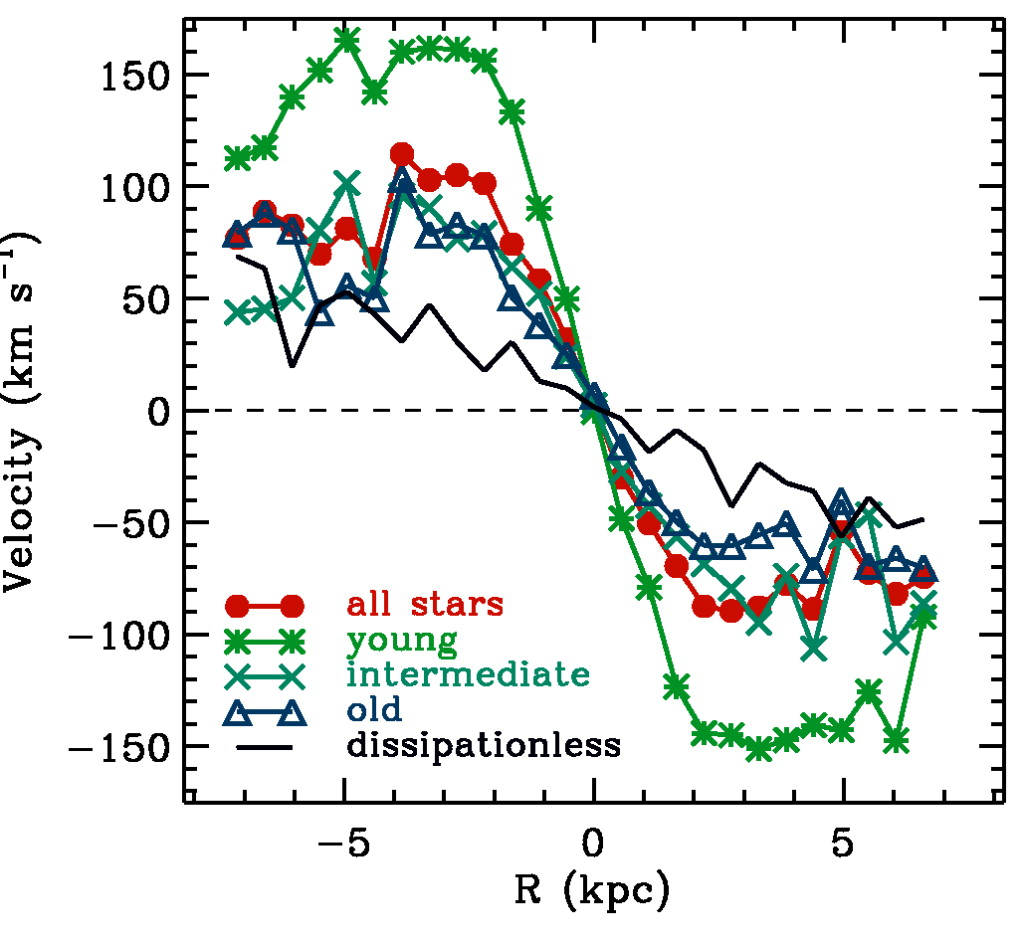
\includegraphics[width=\columnwidth]{RA2/rotationref.jpg}
  \caption{The rotation curve of a simulated disspational major merger remnants, segmented by particle types. The roational velocity is plotted as a function of radius, adapted from \cite{Cox_2006}. The figure shows that old stars retain angular momentum the most, dominating the remnant's rotation structure. }
  \label{fig:rotationref}
\end{figure}


% Paragraph 4: What are the open questions in your chosen topic area (as defined in
% Paragraph 1)? One of these open questions must relate to your specific project. How are people trying to solve these questions? You must include citations.

While these simulations provides strong theoretical studies on future galaxy mergers, key unresolved questions remain : what determines a major merger remnants becomes a fast or slow rotator? What components of galaxies, such as gas content, disk masses, and bulge masses, contributes to the resulting kinematic properties? The MW/M31 system presents an excellent case study to refine our understanding of how major mergers affect galaxy kinematics. By combining observational constraints with detailed numerical simulations such as those simulation \citep{van_der_Marel_2012}, we can develop more precise models of galaxy evolution and rotational transformation.

\section{This Project} 

% Paragraph 1: Introduce your specific project. (e.g. “In this paper, we will study the change in position of the SMBHs of the Milky Way and M31’s throughout the
% future collision and eventual merger of these two galaxies”). This isn’t supposed to be general. Be as specific as you can be.
In this paper, we will investigate the kinematic properties of remnants from future merger between the Milky Way and Andromeda. By focusing on contribution of stellar disk and stellar bulge components on rotational velocities of the remnants, we will study emergence of rotational or dispersion-dominated support. 

% Paragraph 2: Which of the open questions (paragraph 4 of the intro) does this project address?
Out study directly addresses the open question of what components contribution to change in rotation properties throughout merger interaction. By analyzing MW/M31 major merger system, we aim to test theoretical prediction based on observational constraints. The MW and M31 contains significant stellar disks and moderate gas contents. With this system, we can explore future merger system's behavior with specific initial conditions in kinematic perspective. 

% Paragraph 3: Why is this open question an important problem to solve for our understanding of Galaxy Evolution? How will your study help us to address the open question?

\section{Methodology}

% Paragraph 1: Start with an introduction to the simulations you are using. You must
% reference the paper associated with the simulations and describe what is meant by an “N-body” simulation. Describe how each galaxy is initially modeled (Dark matter halo with what profile, disk, etc).

To study the kinematic properties of the MW/M31 merger remnant, we utilize N-body simulations originally developed by \citep{van_der_Marel_2012}. An N-body simulations solves the gravitational interactions between a set of particles, representing a mass contribution in a galaxy. These simulations solves Newton's gravitational law to provide theoretical prediction of future positions and velocities of particles in the system. 



% Paragraph 2: Overview your approach. What particle types are you using, what resolution of the simulation data (VLowRes, LowRes, HighRes).

This work combines individual N-body simulated Low Resolution MW and M31 galaxy data into one dataset, as a remanent. We will analyze the kinematics of the remnant by studying its velocity dispersion by using low resolution simulation at 8.0 Gyrs -- approximately the time when two galaxies completed their merging process and relative velocity has stabilized sufficiently. We focus on stellar disk and stellar bulge contribution to study the internal dynamics of the remnant. Dark matter contribution is included in simulation throughout the merger process, however excluded from analysis on velocities. 

% Paragraph 3: Describe the calculations your code will compute. You must include
% all relevant equations and citations, and describe the meaning behind every parameter
% in the equation (e.g. The circular speed is defined as V 2c = GM/r, where M is the Mass of the host galaxy (M⊙) and r is the Galactocentric radius (kpc) ). Note that the reference for the Hernquist profile is Hernquist 1990 ApJ 356.

In order to determine rotation properties of remnants, we begin by combining MW and M31 data into a single dataset.  We first recalculate the center of mass of the merged system and shift all particle positions and velocities into this new frame. Next, we compute the total angular momentum and rotate the coordinate system to align cartesian z-axis with the angular momentum vector, ensuring that the main rotation occurs in x-y plane. We calculate the rotation curve by computing the azimuthal velocity of particles. To examine the system is rotationally supported or not, we evaluate the ratio of maximum rotation velocity and the velocity dispersion, over a range of radius from the center. The velocity dispersion $\sigma$ is calculated as the variance of the particle velocities: 
\begin{equation}
    \sigma ^2 = \frac{1}{N} \sum_{i=1}^{N} (v- \langle v \rangle)^2 
\end{equation}

\begin{equation}
    \langle v \rangle = \frac{1}{N}  \sum_{j=1}^{N} v_j
\end{equation}
, where $\sigma $ is the variance, $\langle v \rangle $ is mean velocity, $N$ is number of particles in simulation, and $v$ is velocity of each particle. We will implement those using \texttt{NumPy} functions: \texttt{numpy.mean()}, \texttt{numpy.std()}.


% Paragraph 4:: Describe the plots you will need to create and explain why those plots will answer your question. Note that later your results section must feature at least two figures that you created. One Figure can be generated entirely by code from Homeworks or In Class Labs (e.g. phase diagrams, density plots). The other figure must be generated by code that includes one new function or method that YOU created BY YOURSELF.
To visualize the kinematic structure of the remnant, we will generate a figure of the profile of $(V/\sigma)_{max}$ as a function of radius. This plot will help us to understand velocity profiles as a function of radius, revealing the ratio between main coherent rotation of the system and random motion of each particle. Figure 2 is an example of a plot to be created. This figure is essential for answering the question whether the major merger remnant is a fast or slow rotator. The higher value of the $(V/\sigma)_{max}$ profile would suggest the remnant will be the more rotationally supported, higer density towards the center.  


\begin{figure}[h]
  \centering
  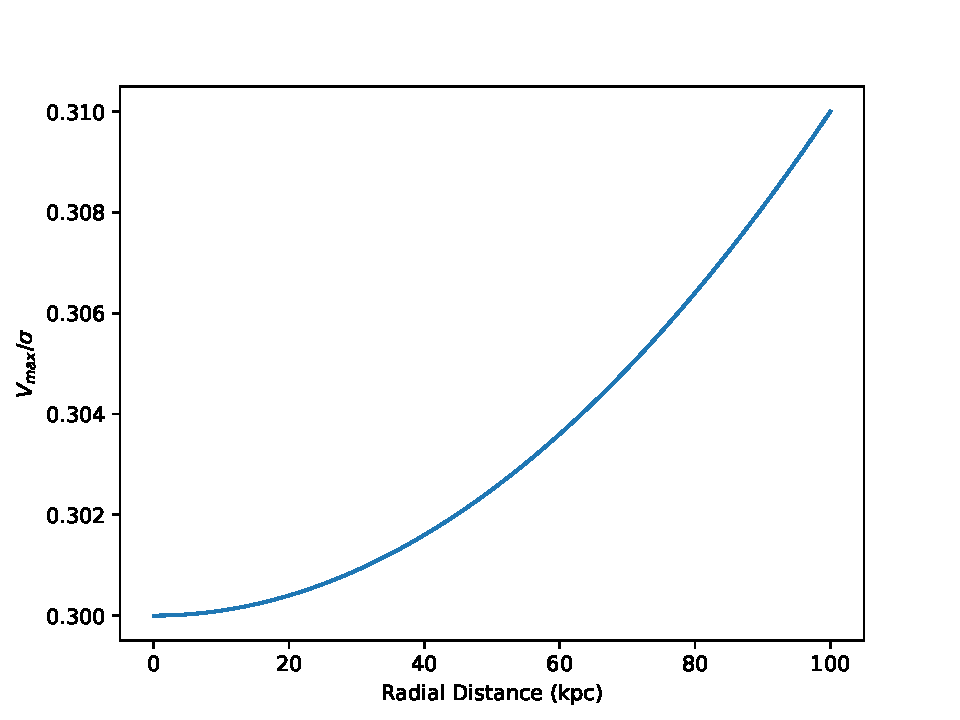
\includegraphics[width=\columnwidth]{RA2/Velocity dispersion profile.pdf}
  \caption{Example of the plot to be made based on analysis. Velocity Dispersion profile $(V/\sigma)_{max}$ as a function of Radial distance from the center in kpc. We expect the ratio to increase as radius increase. }
  \label{fig:lab7example}
\end{figure}






\bibliography{refs}
\bibliographystyle{aasjournal}


\end{document}

